\chapter{Multi-armed Bandit Algorithms}
\label{chapter:MAB}

After identifying the unimodals in Chapter~\ref{chapter:clustering} and defining a ROI for exploitation in Chapter~\ref{chapter:projection},
we still need to decide how to \textbf{allocate our resources}.
During different phases of searching, the \textit{exploration vs. exploitation} dilemma needs to be handled accordingly.
There have been many literatures considering how the algorithms converge 
and how to manipulate the searching step-size in order to find the global optimum more efficiently.
Here, we propose that different strategies should be taken according to \textit{evaluations left}.
Generally, we would like to allow more exploration in the beginning when there are abundant evaluations left.
Then, we would like to gradually increase the portion of exploitation behavior.
When there are very few evaluations left, we should concentrate on exploiting the current best hill.
Therefore, instead of letting the algorithms handle both exploration and exploitation, we propose a bandit technique to help manage the exploration, and leave the simpler subproblems for the algorithms to exploit.

Multi-armed Bandit (MAB) algorithms are suitable for this scenario, 
since it learns model from outcomes and the actions it takes do not change the state of the world.
Moreover, the decisions that it makes help discover more knowledge which can improve future decisions.
This matches our description for exploring fitness landscape in real-valued optimization.
However, our goal is a little bit different since we focus more about obtaining the optimum solution.
Unlike canonical MAB algorithms that minimize regrets, we wish to maximize the probability of gaining the maximum rank.

In the following sections, we'll first describe the MAB problem.
Then, we briefly introduce some MAB algorithms 
that were described in the review which Vermorel et. al. made on MAB algorithms~\cite{Vermorel:2005:MAB}.
Finally, we propose a new bandit technique that aims to maximize the probability of gaining the maximum rank.


\section{The Multi-armed Bandit Problem}

The MAB problem was originally described by Robins in 1985~\cite{Robbins:1985:MAB}.
In this problem, a gambler has to decide which machine to play in a row of slot machines, a.k.a one-armed bandits, and how often to play it.
When the lever is pulled, each machine provides a reward according to a probability distribution.
Therefore, the gambler iteratively plays one lever at each round and observes the probability of reward for each arms.
Here, the gambler is also facing the \textit{exploration vs. exploitation} trade-off.
The problem of determining the best strategy for the gambler is called the Multi-armed Bandit problem.


The MAB problem can be more formally described as 
an agent deciding which one of the $K \in \mathbb{N}_+$ arms to pull at time $t$ to receive the maximum reward.
The $K$ arms can be seen as a set of real distributions $B = \{ R_1, ..., R_K \} $.
Let $\mu_1, ..., \mu_K$ be the mean of rewards for each arm, and $\mu^* = \max_{k} \{ \mu_k \}$ be the highest reward mean.
The \textit{regret} $\rho$ after $T$ rounds is defined as
\begin{displaymath}
\rho = T\mu^* - \sum_{t=1}^{T} r_t,
\end{displaymath}
where $r_t$ is the reward at time $t$.

The goal is to minimize the regret, which represents the expected difference between the total rewards of an optimal strategy,
and the sum of the actual rewards that have been collected.  
The reason for concerning the regret is because we would like to achieve a \textit{zero-regret strategy}.
A \textit{zero-regret strategy} is a strategy whose average regret per round $\rho / T$ tends to zero with probability $1$ 
when the number of played rounds tends to infinity.
The \textit{zero-regret strategy} are guaranteed to converge to an optimal strategy if enough of rounds are played~\cite{Vermorel:2005:MAB}.



\section{Bandit Algorithms Overview}

The $\epsilon$-greedy strategy, first proposed by Watkins~\cite{Watkins:1989:eta}, 
is the simplest and one of the most widely used strategy to solve the MAB problem.
Given an $\epsilon \in (0,1)$,
the $\epsilon$-greedy strategy chooses a random lever with a probability $\epsilon$, 
and chooses the lever with the highest estimated mean with a probability $1 - \epsilon$.
It is also known as \textit{semi-uniform} method since it implies a uniform probability of exploration among a set levers.

There are two variants of the $\epsilon$-first strategy: the $\epsilon$-first strategy and the $\epsilon$-decreasing strategy.
The $\epsilon$-first strategy does pure exploration in the $\epsilon T$ first rounds for a given $T \in \mathbb{N}$.
Then for the remaining $(1 - \epsilon ) T$, it does pure exploitation by pulling the lever with the highest estimated mean.
Another approach is the $\epsilon$-decreasing strategy.
The $\epsilon$ greedy strategy is sub-optimal,
since the factor $\epsilon$ prevents the strategy from getting arbitrarily close to the optimal lever.
Therefore, the $\epsilon$-decreasing strategy adopts a decreasing $\epsilon$ 
for getting arbitrarily close to the optimal strategy asymptotically~\cite{Vermorel:2005:MAB}.
By carefully choosing the $\epsilon$, the $\epsilon$-decreasing strategy can achieve zero regret.

The \textit{SoftMax strategy}, also known as the \textit{Boltzmann exploration}, is first proposed in~\cite{Luce:1959:softmax}.
It chooses the $k$-th lever with probability
\begin{displaymath}
p_k = \frac{ e^{ \hat{ \mu_k } / \tau } }{ \sum_{i=1}^{n} e^{ \hat{ \mu_i } / \tau } },
\end{displaymath}
where $\hat{\mu_i}$ is the estimated reward mean of the $i$-th lever,
and $\tau \in \mathbb{R}_+$ is the \textit{temperature} parameter.


The \textit{interval estimation strategy} is first proposed in~\cite{Kaelbling:1993:interval_estimation}.
It estimates the \textit{optimistic reward} of each lever within a certain confidence interval,
and greedily choose the lever with the highest optimistic mean.
The optimistic reward estimation asymptotically matches the true reward mean as the number of choosing that lever increases.
The optimistic rewards of levers that are not frequently pulled are over-valued, 
and it leads to their exploration as the Interval Estimation strategy greedily choose the lever with the highest optimistic mean.

The Price of Knowledge and Estimated Reward (POKER) strategy~\cite{Vermorel:2005:MAB}
considers three ideas: pricing uncertainty, exploiting the lever distribution and taking into account the horizon
The \textit{pricing uncertainty} is to assign a ``value of information'' to the knowledge acquired by pulling a particular lever.
It is also referred as ``exploration bonuses'' in bandit literatures that helps balancing exploration and exploitation.
The idea behind \textit{exploiting the lever distribution} is that
the properties of unobserved levers could be estimated from the observed levers.
The \textit{horizon} is the number of rounds remain to be played.
Therefore, the ratio between exploration and exploitation should depend on the horizon.
\textit{Taking the horizon into account} can also help to estimate the \textit{price} of the knowledge acquired in POKER.

\section{The New Bandit Technique}

We propose a new bandit technique that aims to maximize the probability of acquiring the best rank in the history.
We only focus on ranks instead of real-valued fitness to generalize the case.

Let $r$ be the probability of not being able to acquire the best point.
Let $m_i$ be the one of the possible models in the arm.
Let $D$ be the model of all the observed data.
The we define the probability of not being able to acquire the best point given a set of observed data as:
\begin{equation}
P(r|D) = \sum_{i} P(r|D, m_i)P(m_i|D) = \sum_{i}P(r|m_i)P(m_i|D).
\end{equation}\label{equation:bandit}
Therefore, we would like find a remain evaluation allocation that gives a minimum probability of not being able to aquire the best point.

\begin{figure}
\centering
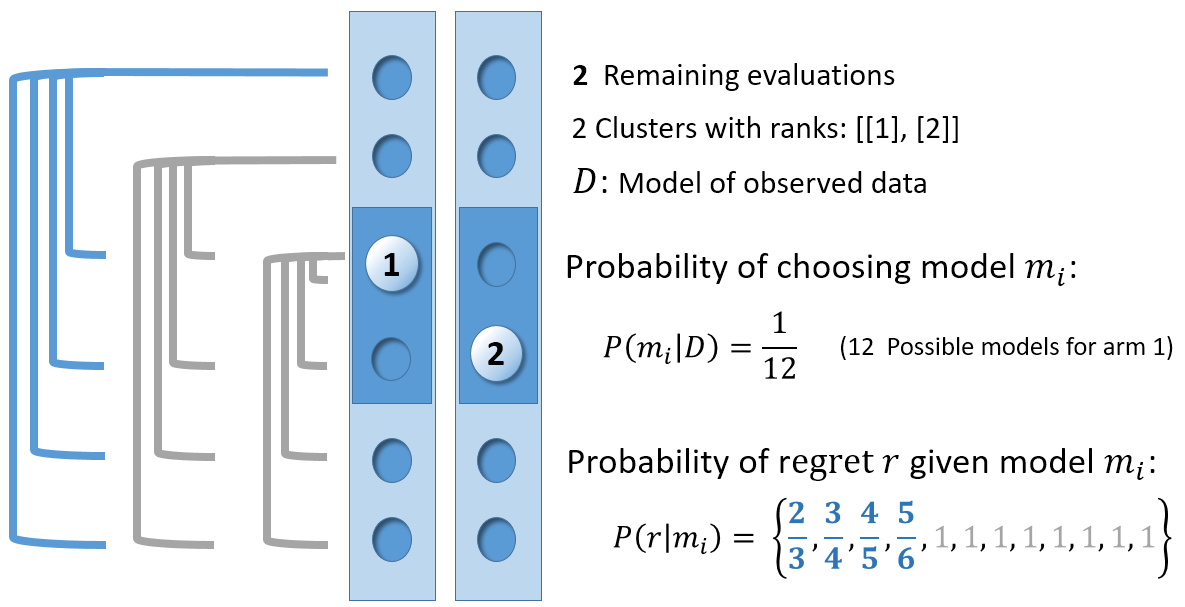
\includegraphics[width=\textwidth]{Bandit_arm}
\caption{Probability of regret.}\label{fig:Bandit_arm}
\end{figure} 

In order to calculate $P(r|D)$, we need to calculate all possible models for an arm with given rank, 
total number of points in the search space, and the number of remain evaluations, 
as shown in Figure~\ref{fig:Bandit_arm}.
The indigo area represents the observed model $D$, 
while the light blue area represents all the possible models given the number of remain evaluations.
It means that if we invest the two remain evaluations on arm 1, 
we might discover two better positions with higher ranks,
or two worse positions that gives fitness worse than the current rank $2$ particle.
That is why there are two possible positions on the top and two on the bottom of each arm.
If the acquired fitness is between the current best and worst particle, 
than the rank would only exchange with another particle in one of the arms,
so no more ``holes'' than the current ranks are needed.
We can find $12$ possible models that matches the current observation, \textit{i.e.} rank $1$ is included.
Therefore, only $4$ out of the $12$ models are possible to acquire the best rank.
We assume the model is uniformly distributed, that is, acquiring different ranks share the same possibility.
We also assume that all models have the same probability to be chosen with the observed data model $D$.
We can then calculate the probability of not being able to acquire the best rank in the clusters.
To demonstrate the idea, we consider the right most blue model that contains the best and the worst possible ranks in Figure~\ref{fig:Bandit_arm}.
The probability of not acquiring the best model for that specific model $m_i$ is $P(r|m_i) = 5/6$,
while the probability for choosing that model is $P(m_i|D) = 1/12$.
Similarly, we can calculate the probability of regret for all models.


\begin{figure}
\centering
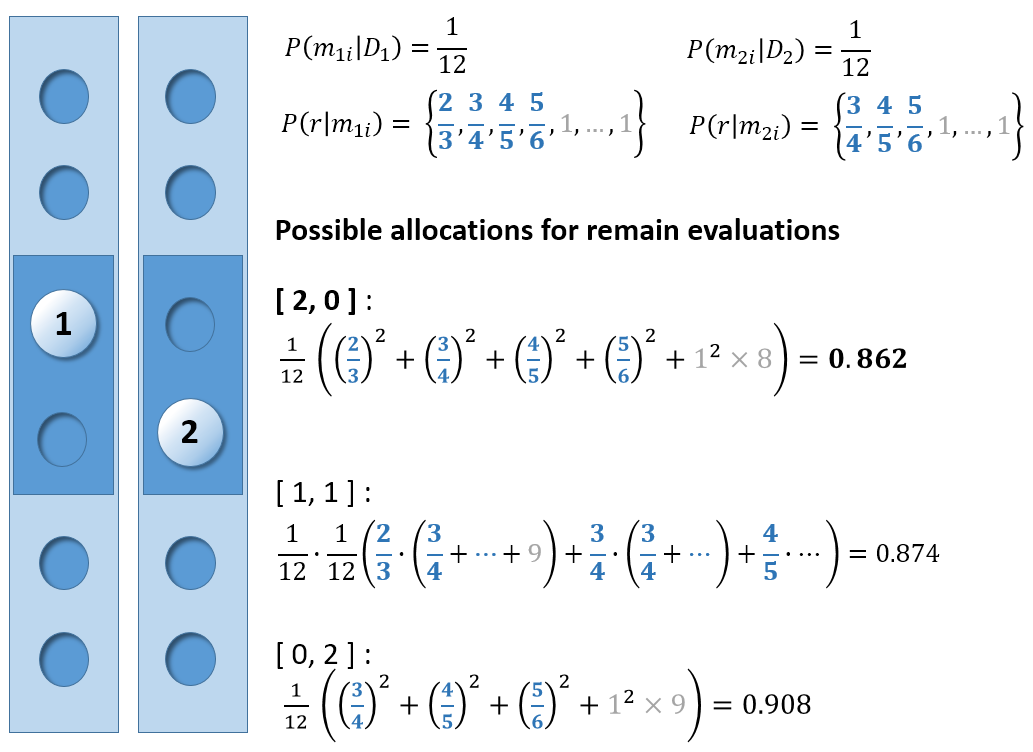
\includegraphics[width=\textwidth]{Bandit_regret}
\caption{Probability of regret for all allocation combinations.}\label{fig:Bandit_regret}
\end{figure} 
Given all the models and their corresponding probability of not acquiring the best rank, 
we can use Equation~\ref{equation:bandit} to calculate the total probability of regret given a set of remain evaluations allocation.
For example, if we decide to invest both of the remaining evaluations on the first arm,
then the probability of not acquiring the best model for the right most model would be $P(r|m_i) = (5/6)^2$,
while the probability for choosing that model is still $P(m_i|D) = 1/12$.
Therefore, we can calculate the probability of regret as illustrated in Figure~\ref{fig:Bandit_regret}.
After calculate the probability of regret all possible combinations, \textit{i.e.} [2,0], [1,1], [0,2], 
we select the evaluation allocation model with the minimum regret.
In this case, it is to invest all the remaining evaluations on the first cluster.
This result satisfies our assumption that in the end with few evaluations left, 
one should focus on exploiting the current best hill.
If today there are still lots of evaluations left, 
this technique gives an even evaluation allocation that only slightly favors the current best arm.
This also satisfies our assumption that in the beginning, we should explore evenly between all possible clusters.


